\documentclass[11pt,a4paper]{article}

\usepackage[T1]{fontenc}
\usepackage[utf8]{inputenc}
\usepackage[margin=2.4cm]{geometry}
\usepackage{graphicx}
\usepackage{amsmath,amssymb}
\usepackage{bm}
\usepackage{hyperref}
\usepackage{xcolor}
\usepackage{siunitx}
\usepackage{booktabs}
\usepackage{natbib}
\usepackage{caption}
% Resolve references to the separate supplement (Figs.~S1, S2); needs
% supplement.aux, so the Makefile compiles both files (twice).
\usepackage{xr-hyper}
\externaldocument{supplement}

\captionsetup{font=small,labelfont=bf,labelsep=period,justification=raggedright,singlelinecheck=false}

\hypersetup{colorlinks=true, linkcolor=blue!50!black, citecolor=blue!50!black, urlcolor=blue!50!black}

\graphicspath{{figures/}}

\begin{document}

\title{Density-gated noise rectification in a Vicsek--Couzin flock: one dense-phase mechanism, additive at matched decorrelation}

\author{Yaya Youssouf Yaya \quad Mamadou Sy\thanks{D\'epartement de
        Math\'ematiques et Informatique and Laboratoire d'Analyse
        Num\'erique et Informatique, Universit\'e Gaston-Berger de
        Saint-Louis, S\'en\'egal. \texttt{mamadou.sy@ugb.edu.sn}} \\[0.5em]
        \small D\'epartement de Math\'ematiques, \'Ecole Normale Sup\'erieure de
               N'Djam\'ena, BP~206, N'Djam\'ena, Tchad \\
        \small Chercheur Associ\'e, LMA, U.F.R.~Sciences et Technologies,
               Universit\'e Assane Seck de Ziguinchor, BP~523, Diabir,
               Ziguinchor, S\'en\'egal \\
        \small \texttt{yy.y@zig.univ.sn} \;\;
               ORCID: \href{https://orcid.org/0000-0003-0781-4923}{0000-0003-0781-4923}}

\date{\today}

\maketitle

\begin{abstract}
Flocking models hold the self-propulsion speed and the
angular-noise distribution fixed as global constants. Active
matter has relaxed each of them on its own: a density-dependent
speed drives motility-induced phase separation, and heavy-tailed
L\'evy reorientations are reported in bacteria, in foragers and
in migrating cells. What has not been tested is whether the two
reinforce each other when one cue drives both, and the question
is as much methodological as physical, since apparent cooperation
between adaptive channels is easy to manufacture and hard to rule
out. We therefore gate the speed and the stability index of a
wrapped $\alpha$-stable kick through a single sigmoid in the
local neighbour count, so that a crowded particle is at once slow
and Gaussian-like and an isolated one fast and Cauchy-like: the
arrangement most favourable to a synergy. None survives.
Heavy-tailed reorientations alone grow no size-dependent
susceptibility; only the motility channel builds a
phase-separated dense phase, and the noise-shape channel acts
solely inside it, rectifying wrapped Cauchy kicks into Gaussian
ones. The apparent super-additivity comes from comparing modes at
matched nominal noise amplitude instead of matched effective
decorrelation: equalise the effective rate and the susceptibility
excess is gone, while the dense static and dynamic correlation
gaps reverse sign, leaving two channels that simply add. The
coupling thus reduces to a density-gated lowering of the
dense-phase effective noise, set by the motility threshold alone
and contingent on a metric kernel. The lesson travels beyond this
model: heavy-tailed and Gaussian dynamics have to be compared at
matched decorrelation, not matched amplitude, or additivity will
be read as synergy.
\end{abstract}

\section{Introduction}

The Vicsek model \citep{Vicsek1995} freezes two ingredients that
real collectives keep fluid: every particle moves at the same
speed, and every reorientation is drawn from the same Gaussian.
Neither assumption survives contact with data. The sign of the
departure, on the other hand, varies from system to system, and
that variability is part of the evidence rather than a detail to
be smoothed over. Motility does respond to crowding, and it
responds downward in confluent tissue and in traffic: epithelial
monolayers slow as they approach jamming
\citep{Angelini2011, Bi2016}, and vehicular flow carries a
pronounced speed--density anti-correlation \citep{Greenshields,
LWR}. In bacterial suspensions and swarms the sign reverses,
hydrodynamic and steric coupling raising the mean swimming speed
as density grows \citep{Colin2019, Beer2020}; even in monolayers
the slowdown has been traced to the maturation of cell--cell
contacts rather than to density as such \citep{Garcia2015}. The
turning statistics are no closer to a fixed Gaussian. Heavy-tailed
L\'evy reorientations are documented in foragers, T~cells and
swarming bacteria \citep{Reynolds2018, Harris2012, Ariel2015,
Zaburdaev2015}, and crowding reshapes those too: cell density
suppresses the reversal frequency of \emph{Myxococcus xanthus}
through contact-dependent signalling \citep{Shi1996}, raises the
effective reorientation rate of \emph{Escherichia coli} in dense
suspensions \citep{Colin2019}, and shifts the L\'evy exponent of
swarming trajectories as a swarm densifies \citep{Beer2020}. Even
there the interpretation is contested, the best-studied case of a
density-driven L\'evy-to-Brownian shift having been attributed to
passive encounter statistics rather than to any change of
movement strategy \citep{deJager2014}. A flocking model in which
both inputs read the local environment is therefore closer to the
biology than one that fixes either, even if no single organism is
known to realise the particular combination we study.

These two relaxations have so far been pursued apart. On the
motility side, a steep enough density-dependent speed drives
motility-induced phase separation (MIPS) with no alignment at all
\citep{TailleurCates2008, Fily2012, Redner2013, CatesTailleur2013,
Stenhammar2014, CatesTailleur2015}, now a standard route to
clustering in active matter, and the same slowdown underlies
motility-driven jamming in tissue \citep{Bi2016}. That channel has
already been combined with alignment, which bears directly on
what follows: \citet{Farrell2012} couple a
density-dependent motility to polar alignment and obtain bands and
asters, while \citet{Solon2015PRL} and \citet{Solon2015PRE} show
that the banded state of flocking models is a microphase
separation sustained by nonequilibrium fluctuations. Our
motility-only ablation belongs to that established line and we
treat it as a reference point rather than as a finding. On the
noise side, the Vicsek
lineage has established that how the noise is implemented, and
not merely how large it is, governs the transition: angular and
vectorial noise behave differently and carry very different
crossover sizes \citep{Chate2008, Chate2008EPJB}, the apparent
order of the transition turns on that choice
\citep{Aldana2007, ChateComment2007, Nagy2007, Baglietto2009},
and the measured exponents are not universal but drift with
speed, density and interaction radius \citep{Cambui2016,
Baglietto2008, Baglietto2012, Holubec2021}. Alignment has
likewise been combined with active, non-thermal fluctuations
\citep{Grossmann2012, MartinGomez2018} and recast in spin
language to sharpen the transition question \citep{Solon2013},
while heavy-tailed angular noise has run on its own L\'evy-driven
track \citep{Eliazar2003, Ariel2015, Beer2019}. Across all of it,
and in the reviews that organise the field
\citep{Chate2020, Vicsek2012, Marchetti2013, Bechinger2016}, the
self-propulsion speed and the noise statistics remain independent
modelling choices, each varied while the other is held fixed.

Three things are consequently missing, and they compound. The
first is empirical: no collective has been shown to co-regulate
its motility and the \emph{tail shape} of its turning noise
through a single cue. Density is known to co-regulate speed and
reorientation rate \citep{Colin2019}, to shift heavy-tail
exponents \citep{Beer2020} and to set reversal frequency
\citep{Shi1996}, but joint regulation of speed and tail shape is
an extrapolation from those observations rather than one of them,
which is why we treat the shared sensor below as a deliberate
limiting case and not as a documented mechanism.

The second gap, on the modelling side, is narrower than it may
appear and worth stating precisely, because a
density-dependent noise \emph{amplitude} is not new. The
vectorial-noise update of \citet{Gregoire2004} has been
implicitly neighbour-count dependent since its introduction;
\citet{Frouvelle2012} makes both the alignment rate and the noise
intensity functions of the local density at the kinetic level;
\citet{Haghsheno2024} scales the angular-noise strength directly
by the neighbour count; and \citet{ChenMa2016} lets local density
switch a discrete behavioural mode. What none of these varies is
the \emph{shape} of the turning law. \citet{Clusella2021} come
closest, generalising Vicsek to an arbitrary angular-noise
distribution that may in principle depend on the neighbour count,
and then set that dependence aside explicitly as beyond their
scope; their distributions are thin-tailed and their speed
constant. Our contribution occupies precisely that declined cell.
Making the tail index of the turning law a function of local
density, and coupling it to a density-dependent speed, lets us
ask directly whether the two channels reinforce, cancel or simply
add. The question has content, because the
two channels meet inside the dense regions a flock builds: the
noise distribution sets how a particle escapes a local structure,
and the density-dependent speed builds that structure in the
first place.

The third gap weighs most on what follows, and it is one of
protocol rather than of ingredients. Noise shapes in this
literature are compared at matched nominal amplitude, whereas a
wrapped $\alpha$-stable kick of scale $\eta$ decorrelates a
heading at the rate $\Gamma = 1 - \exp(-\eta^{\alpha})$
\citep{Gatto2003, Pewsey2008, Mardia2000}, a quantity that
depends on $\alpha$ as strongly as it does on $\eta$. Varying
$\alpha$ at fixed $\eta$ therefore varies the effective noise
along with its shape, so any cooperation inferred from such a
comparison is confounded before it is measured. Closing the first
two gaps without controlling for the third would only reproduce
that confound at greater computational expense, and it is the
control, as much as the coupling, that this paper is about.

We couple the two adaptations in the most economical way
available: a single sigmoid in the local neighbour count gates
both the self-propulsion speed and the stability index of a
wrapped $\alpha$-stable angular kick, so a crowded particle is at
once slow and Gaussian-like and an isolated one fast and
Cauchy-like. The stability index sets how heavy-tailed the
turning is, the Cauchy limit ($\alpha = 1$) sprinkling in
occasional near-reversals while the Gaussian limit ($\alpha = 2$)
keeps every turn small, and we treat the $\alpha = 1 \to 2$
interpolation as a family bracketing those two limits rather than
as a fit to any organism. Locking both channels to one cue is
deliberate. It is the arrangement most favourable to a synergy:
if cooperation between an adaptive speed and an adaptive noise
shape exists anywhere in this family, it has its best chance of
appearing here, which is what makes a negative answer
informative. There is no attraction zone, so spatial cohesion
comes entirely from the density-dependent motility rather than
from a cohesive term, and turning both channels off recovers the
original Vicsek dynamics. Two single-channel ablations, a
motility-only mode with adaptive speed and fixed Cauchy noise and
a noise-shape-only mode with fixed speed and Cauchy-to-Gaussian
noise, isolate each contribution against a shared heavy-tailed
reference on a single code path, and a nine-size finite-size scan
at fixed density ($\rho_0 = 2.22$, $L = 15$ to $256$, ten seeds
per size) places the four heavy-tailed modes and the Gaussian
Vicsek baseline on the same footing, with the qualitative split
reproduced away from that density at $\rho_0 = 1.0$ and $3.0$.

The two channels separate cleanly, and only those carrying the
density-dependent speed respond to system size at all. The Cauchy
reference and the noise-shape-only mode return slopes
statistically indistinguishable from zero ($a = -0.03$,
$[-0.07, +0.01]$ and $a = -0.02$, $[-0.05, +0.01]$), so
heavy-tailed reorientations on their own grow no size-dependent
susceptibility, their rare bursts washed out among the many
neighbours of a dense patch; the motility-only ablation does grow
one ($a = +1.04$, $[+0.97, +1.22]$) and the full mode a steeper
one ($a = +1.49$, $[+1.43, +1.68]$). That full-mode value calls
for a comparison with the literature, not a bare report:
$+1.49$ is statistically indistinguishable from
the $\gamma/\nu = 1.45(2)$ established for the standard Vicsek
model \citep{Baglietto2008, Baglietto2012} on the same
$\chi = N\,\mathrm{Var}(\varphi)$ convention, whereas the
motility-only slope excludes it. We read that agreement as a
consistency check and not as evidence of criticality, since the
accompanying diagnostics point the other way: the susceptibility
peak $\eta^\ast(L)$ drifts toward the small-$\eta$ boundary
instead of converging on a fixed $\eta_c$, no data collapse can
be constructed, the Binder cumulant never crosses, and the window
$L = 15$ to $256$ straddles rather than clears the crossover size
$L^\ast \simeq 128$ reported for angular noise at this density
\citep{Chate2008}. We therefore report these slopes as effective
growth rates of a phase-separation susceptibility, bounded above
by the $d = 2$ ceiling $\chi_{\max} \sim N$ that a single dense
domain would saturate, rather than as asymptotic exponents.

Compared at each mode's own near-critical noise, the noise-shape
adaptation then appears to lend the motility-driven growth a
super-additive boost, an excess $\Delta_9 = +0.45$ with a $95\%$
seed-bootstrap interval $[+0.31, +0.60]$. That excess does not
survive the control the effective-noise argument demands.
Retuning the motility-only mode so that its heavy-tailed kick
decorrelates as fast as the full mode's rectified one drives the
excess to $\Delta_9 = +0.02$, additive within error, and reverses
the dense static and dynamic correlation gaps in the same stroke,
the dense $g(r)$ gap going from $+0.153$ to $-0.07$ and the
$C(\tau)$ gap from $+0.13 \ldots +0.24$ to
$-0.08 \ldots -0.42$ as the global retune over-quiets the dilute
phase. What looked like cooperation was a difference in effective
noise, so the two channels act through one local route and, at
matched decorrelation, simply add.

What the noise-shape channel does instead is local, and it can be
counted. Inside the dense phase the shared sigmoid pushes
$\alpha$ toward $2$, and because the kick enters the heading
modulo $2\pi$ the heavy tail acts through the fraction of kicks
that overshoot a half-turn and wrap, $P(|\xi| > \pi) \simeq
0.20\,\eta$ in the Cauchy limit, which is $1.0\%$ to $6.1\%$
across $\eta = 0.05$ to $0.3$ against less than $10^{-11}$ for
the Gaussian limit at the same scale. Driving $\alpha$ from $1$
to $2$ removes precisely this wrapped-uniform fraction, so the
Cauchy bursts that would otherwise scramble a slow particle's
alignment are rectified into coherent kicks: the dense-quartile
heading correlation gains $\Delta g = +0.153$ over the
motility-only ablation while the dilute quartile shows no gap,
the dense mass fuses into fewer and larger clusters, and
$s_{\rm sep}$ rises from $\simeq 1.2$ for the fixed-speed
references to $\simeq 1.7$. A decoupled-sigmoid analysis
(Sec.~\ref{sec:decoupled}) then pins the control variable, the
motility threshold alone setting the sign and amplitude of the
rectification ($R^2 = 0.88$ for bands of constant
$n_\star^v$ against $0.28$ for a sequential-timing alternative)
with the noise-shape threshold passive, and identifies the metric
kernel as a precondition, that dominance weakening to
$R^2 = 0.68$ under topological alignment \citep{Ballerini2008,
Ginelli2010}. The density-triggered slowdown is thus the
precondition throughout: without the dense phase it builds, the
heavy-tailed rectification has nothing to act on and erodes
coherence instead of creating it. We report the internal
falsifications alongside, since they bound the claim as much as
the positive results do: hysteresis is negligible, the
band-soliton index stays at $b \le 1.06$ so no travelling band
ever forms, and the dense patches consolidate spatially without
living any longer ($1.60$ against $1.57$ snapshots, $p = 0.08$).

Section~\ref{sec:model} defines the two-feedback model, its
ablations and the numerical protocol, and states the
matched-decorrelation control on which the rest of the paper
leans. Section~\ref{sec:results} reports the global diagnostics,
the parametric analyses and the local diagnostics (heading
correlations, cluster statistics, single-particle dynamics and
the decoupled-sigmoid dissection) that localise the rectification
to the dense phase. Section~\ref{sec:disc} discusses the
mechanism, its place in the literature and its limits, and the
appendix (Sec.~\ref{sec:hydro}) sketches a heuristic
hydrodynamic account of the dense-phase rectification.

\section{Model and methods}
\label{sec:model}

\subsection{Dynamics}

$N$ point particles live in a square box of side $L$ with
periodic boundaries; particle $i$ carries a position $\mathbf
x_i \in [0, L)^2$ and a heading $\theta_i \in (-\pi, \pi]$,
advanced synchronously through
\begin{equation}
\theta_i(t+1) = \bigl[\theta_i^\star(t+1) + \xi_i(t)\bigr]
   \bmod 2\pi,
\qquad
\mathbf x_i(t+1) = \mathbf x_i(t) + v_i(t+1)\,\vec e_i(t+1)
   \pmod L,
\label{eq:update}
\end{equation}
with $\vec e_i = (\cos\theta_i, \sin\theta_i)$. The desired
heading $\theta_i^\star$ follows the Couzin priority rule
\citep{Couzin2002} with the repulsion set $\mathcal R_i =
\{j \neq i : |\mathbf r_{ij}| < R_r\}$,
$\mathbf r_{ij} = \mathbf x_j - \mathbf x_i$, and the
alignment set $\mathcal A_i = \{j \neq i : R_r \le
|\mathbf r_{ij}| < R_a\}$, both sensed omnidirectionally.
There is no attraction zone: spatial cohesion comes
entirely from the density-dependent motility (the MIPS
route), not from a Couzin cohesion term, and ``Couzin'' here
labels only the zonal priority rule of repulsion over alignment
over inertia:
\begin{equation}
\theta_i^\star(t+1) =
\begin{cases}
\arg\!\left(-\sum_{j \in \mathcal R_i}
   \mathbf r_{ij} / |\mathbf r_{ij}|\right),
   & \mathcal R_i \neq \emptyset, \\[4pt]
\arg\!\left(\sum_{j \in \mathcal A_i} e^{i\theta_j(t)}\right),
   & \mathcal R_i = \emptyset
   \text{ and } \mathcal A_i \neq \emptyset, \\[4pt]
\theta_i(t),
   & \mathcal R_i = \mathcal A_i = \emptyset.
\end{cases}
\label{eq:theta_star}
\end{equation}
Interactions run in $O(N)$ on a cell-list partition.

The angular kick $\xi_i$ is a symmetric $\alpha$-stable variate
with a particle-dependent stability index,
\begin{equation}
\xi_i(t) \sim S_{\alpha_i(t)}\bigl(c = \eta,\, \beta_{\rm stab}
   = 0,\, \mu = 0\bigr),
\label{eq:noise}
\end{equation}
sampled with the Chambers--Mallows--Stuck representation
\citep{Chambers1976} in the parametrisation of
\citet{Samorodnitsky1994} and \citet{Nolan2020}. The Gaussian
limit $\alpha_i = 2$ is handled separately and recovers the
original Vicsek noise. Since the kick is added to a heading and
reduced modulo $2\pi$, the law that actually acts on the dynamics
is the \emph{wrapped} symmetric $\alpha$-stable distribution
\citep{Gatto2003, Pewsey2008, Mardia2000}, whose mean resultant
length $\langle\cos\xi\rangle = \exp(-\eta^{\alpha})$ we use
throughout as the effective decorrelation scale; the consequences
of that wrapping for the comparison between modes are developed in
Sec.~\ref{sec:hydro}.

\subsection{The shared sigmoid}

The single departure from canonical Vicsek dynamics is that
both the speed and the noise stability index become local
fields, controlled by the same neighbour count $n_i(t) =
|\mathcal A_i(t)|$ through one sigmoid,
\begin{align}
\sigma_i(t) & = \frac{1}{1 + \exp\bigl[-s\,(n_i(t) -
   n_\star)\bigr]},
\label{eq:sigmoid} \\
v_i(t) & = v_{\max} - (v_{\max} - v_{\min})\,\sigma_i(t),
\label{eq:v_adapt} \\
\alpha_i(t) & = \alpha_{\min} + (\alpha_{\max} - \alpha_{\min})
\,\sigma_i(t).
\label{eq:alpha_adapt}
\end{align}
A crowded particle ($n_i \gg n_\star$) sits at $\sigma_i \to
1$, $v_i \to v_{\min}$, $\alpha_i \to \alpha_{\max} = 2$; an
isolated one ($n_i \ll n_\star$) at $\sigma_i \to 0$, $v_i \to
v_{\max}$, $\alpha_i \to \alpha_{\min} = 1$. The two channels
are locked, slow meaning Gaussian and fast Cauchy
(Fig.~\ref{fig:schematic}).

\begin{figure}[htbp]
    \centering
    
\includegraphics[width=0.32\linewidth]{fig_setup_geometry.pdf}\hspace{2pt}%
    
\includegraphics[width=0.32\linewidth]{fig_setup_noise.pdf}\hspace{2pt}%
    
\includegraphics[width=0.32\linewidth]{fig_setup_sigmoid.pdf}\\[2pt]
    
\includegraphics[width=0.32\linewidth]{fig_setup_inertia.pdf}\hspace{2pt}%
    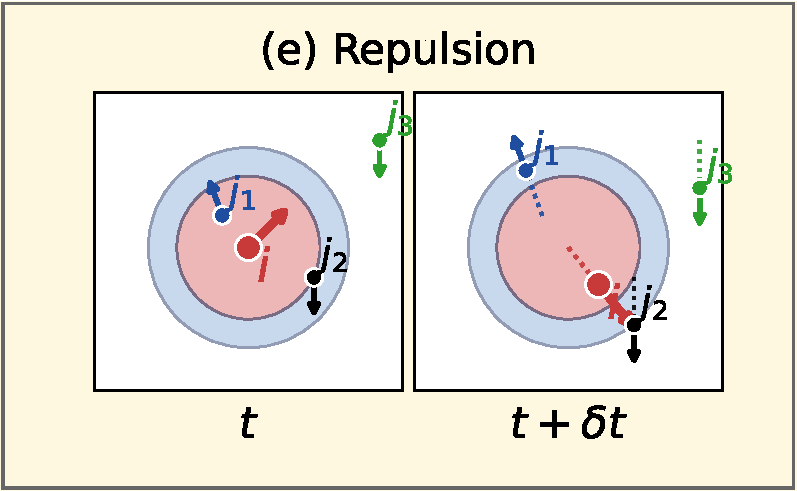
\includegraphics[width=0.32\linewidth]{fig_setup_repulsion.pdf}\hspace{2pt}%
    
\includegraphics[width=0.32\linewidth]{fig_setup_alignment.pdf}
    \caption{Vicsek--Couzin setup and update rules. (a) Two-zone
    geometry around a focal particle: repulsion disc ($d < R_r$),
    alignment annulus ($R_r \leq d < R_a$), full $360^\circ$ vision,
    priority repulsion $\to$ alignment $\to$ inertia. (b) Symmetric
    $\alpha$-stable noise pdfs; smaller $\alpha$ narrows the bulk
    and heavies the tails. (c) The shared sigmoid: $n_i$ sets both
    $v_i$ (purple) and $\alpha_i$ (green), so a crowded particle is
    slow and Gaussian, an isolated one fast and Cauchy. (d)--(f)
    Worked inertia, repulsion and alignment steps of
    Eq.~\eqref{eq:theta_star}, each at $t$ and $t + \delta t$. The
    shared sigmoid is the one departure from canonical Vicsek
    dynamics.}
    \label{fig:schematic}
\end{figure}

\subsection{Reference and ablation modes}

The two-feedback model (\emph{double-adaptive}) runs against
three controls on the same code path. Setting $v_{\min} =
v_{\max}$ and $\alpha_{\min} = \alpha_{\max} = 2$ recovers the
original Vicsek dynamics (\emph{Vicsek reference}); setting
instead $\alpha_{\min} = \alpha_{\max} = 1$ gives the
heavy-tailed \emph{Cauchy reference}, the backdrop on top of
which the feedbacks switch on. The \emph{noise-shape only} mode
activates the noise-shape channel with $v_i$ frozen at
$v_{\max}$; the \emph{motility only} mode activates the motility
channel with $\alpha_i$ frozen at the Cauchy value.

\subsection{Order parameters and observables}

The instantaneous polar order parameter is $\varphi =
\frac{1}{N}\big|\sum_i e^{i\theta_i}\big|$, and the polar order
parameter we report is its average,
\begin{equation}
\langle\varphi\rangle = \Big\langle \frac{1}{N}
   \big|\textstyle\sum_i e^{i\theta_i}\big|\Big\rangle,
\end{equation}
the susceptibility its scaled variance $\chi = N\,
\mathrm{Var}(\varphi)$, and the Binder cumulant $U_4 = 1
- \langle\varphi^4\rangle / (3 \langle\varphi^2\rangle^2)$
\citep{Binder1984}, which we read with caution since every mode
(the Cauchy reference included) drives it to the same
$0.28$--$0.31$ dip and on its own it does not diagnose the
transition here. For spatial phase separation we use
\begin{equation}
s_{\rm sep} \equiv \max_{\rm bins}\frac{n_{\rm bin}}
   {\mathrm{med}(n_{\rm bin})},
\label{eq:s_sep}
\end{equation}
the ratio of the densest grid cell to the median cell on a
$10 \times 10$ partition: a homogeneous fluid sits at
$s_{\rm sep} \simeq 1$, a phase-separated configuration well
above, and a grid-free pair-correlation analogue (the
$95$th-percentile / median ratio of the per-particle local
density within radius $R = 1$) ranks the modes the same way. To
separate a traveling band from an isotropic patch we use the
band-soliton index,
\begin{equation}
b \equiv \frac{\max_{x_\parallel} \rho(x_\parallel)}
   {\langle\rho\rangle},
\label{eq:b}
\end{equation}
the maximum of the time-averaged density profile along the
instantaneous polar-flow axis $x_\parallel$ divided by the
spatial mean. A metric-Vicsek traveling band gives
$b \gtrsim 1.5$; an isotropic patch gives $b \simeq 1$.

\subsection{Numerical protocol}

The finite-size scan spans nine sizes
$L \in \{15, 22, 30, 45, 64, 90, 128, 180, 256\}$ at fixed
density $\rho_0 = N/L^2 = 2.22$ (up to $N \simeq 1.5\times10^5$
particles), with $1500$ warm-up and $1000$ measurement steps
from $\theta_i \equiv 0$. The
load-bearing slopes (Table~\ref{tab:slopes} and the
$\chi_{\max}(L)$ panel of Fig.~\ref{fig:pilot}) come from a
homogeneous protocol with ten seeds at \emph{every} size, so the
bootstrap intervals rest on a uniform replication budget, while the
$\eta$-resolved diagnostic curves (the remaining panels of
Fig.~\ref{fig:pilot}) use three seeds per
$(\mathrm{mode}, L, \eta)$ cell. To separate a robust
phase-separation split from a parameter-window effect we repeat
the scan at $\rho_0 \in \{1.0, 3.0\}$ (sizes $22$ to $128$). The
noise grid is
$\eta \in \{0.005, 0.010, 0.020, 0.035, 0.050, 0.075, 0.100,
0.150, 0.200, 0.300\}$, and the fixed parameters are $R_r =
0.5$, $R_a = 0.7$, $n_\star = 3$, $s = 2$, $v_{\min} = 0.005$,
$v_{\max} = 0.05$, $\alpha_{\min} = 1$, $\alpha_{\max} = 2$. The
interaction loop is numba-JIT compiled. A small-$\eta$
refinement $\{0.001, 0.002, 0.003, 0.0075\}$ at the first five
sizes (two seeds) confirms that $\chi_{\max}$ does not lurk
outside the original window, bar the noise-shape-only ablation
at $L = 45$, which we report with its updated value.

\section{Results}
\label{sec:results}

A visual reference fixes intuition before the diagnostics. We
compare motility-only and double-adaptive configurations at
$\rho_0 = 2.22$ across three sizes $L \in \{30, 90, 128\}$ and
three noise levels spanning the ordered ($\eta = 0.020$),
near-critical ($\eta = 0.10$) and disordered ($\eta = 0.30$)
regimes (Fig.~\ref{fig:snapshot}). Deep in the ordered phase the
flock is almost fully aligned in both modes; at near-critical
$\eta$ it breaks into locally ordered slow patches in a faster
disordered gas; at $\eta = 0.30$ the particles fill the box with
no coherent heading. The near-critical column is the operating
point at which the rectification is active, and there the
double-adaptive panels hold a tighter dense core than their
motility-only neighbours at every size.

\begin{figure*}[htbp]
    \centering
    
\includegraphics[width=\linewidth]{fig_double_snapshot.pdf}
    \caption{Real-space configurations at $\rho_0 = 2.22$, single
    seed, after $3000$ warm-up steps, three sizes
    $L \in \{30, 90, 128\}$ (one row each). Per row the noise runs
    left to right: (a) $\eta = 0.020$ (ordered), (b) $\eta =
    0.10$ (near-critical), (c) $\eta = 0.30$ (disordered); each
    placing motility-only left of its double-adaptive counterpart.
    Arrows are coloured by local speed $v_i$ (shared colorbar), a
    deliberate departure from a geometry-only snapshot because
    the speed field is the control variable, with
    a $5 \times 5$ zoom inset and the polar order
    $\langle\varphi\rangle$ per panel.}
    \label{fig:snapshot}
\end{figure*}

\subsection{Global diagnostics}
\label{sec:results-global}

\subsubsection{Finite-size scaling of the susceptibility}

To see whether the two adaptations leave a thermodynamic trace
we run all four heavy-tailed modes on the nine-size grid of
Sec.~II~E and read the susceptibility peak $\chi_{\max}(L)$,
its slope $a$ in $\chi_{\max} \sim L^a$ separating them
(Fig.~\ref{fig:pilot}, Table~\ref{tab:slopes}).

\begin{figure}[htbp]
    \centering
    
\includegraphics[width=0.95\linewidth]{fig_double_pilot.pdf}
    \caption{FSS diagnostics, four modes: Cauchy reference (blue),
    noise-shape only (green), motility only (red), double-adaptive
    (purple). The $\eta$-resolved panels (three seeds) show, versus
    $\eta$ at the largest pilot size $L = 128$: (a) polar order
    $\langle\varphi\rangle$, (b) susceptibility $\chi$, (c)
    $s_{\rm sep}$, (d) Binder cumulant $U_4$; (e) log--log
    $\chi_{\max}$ versus $L$ with fitted slopes, over the nine
    homogeneous sizes ($L = 15$ to $256$, ten seeds) of
    Table~\ref{tab:slopes}; (f) mean speed
    $\langle v_i\rangle$ (solid) and mean stability
    $\langle\alpha_i\rangle$ (dotted).}
    \label{fig:pilot}
\end{figure}

The slopes split cleanly into two regimes. The three
fixed-noise-shape modes (Vicsek--Gaussian, Cauchy, noise-shape
only) carry slopes indistinguishable from zero ($-0.03$,
$-0.03$, $-0.02$), every $95\%$ interval straddling the origin
($[-0.05, +0.01]$, $[-0.07, +0.01]$, $[-0.05, +0.01]$): none
grows a size-dependent susceptibility on the nine-point lever,
the Cauchy-reference $\chi_{\max}$ staying flat near unity. The
two motility-active modes do grow one:
$a_{\rm motility} = +1.04$ ($[+0.97, +1.22]$) and $a_{\rm full}
= +1.49$ ($[+1.43, +1.68]$), the full mode steeper and the
intervals disjoint. These are growth rates of a
phase-separation susceptibility, not critical exponents:
extending the lever from seven to nine sizes lowers both slopes
($a_{\rm motility}: +1.29 \to +1.04$, $a_{\rm full}: +1.95 \to
+1.49$), so the apparent exponent is not stable, and a
single phase-separated domain would saturate at the
$d = 2$ ceiling $\chi_{\max} \sim N$; we find neither a data
collapse nor the $U_4$ crossing a genuine critical point would
require. The synergy diagnostic
\begin{equation}
\Delta \equiv (a_{\rm full} - a_{\rm Cauchy})
   - (a_{\rm noise} - a_{\rm Cauchy})
   - (a_{\rm motility} - a_{\rm Cauchy})
\label{eq:delta}
\end{equation}
vanishes for two linearly-combining channels above the Cauchy
backdrop. With the Cauchy and noise-shape slopes both
essentially zero, $\Delta_n$ (on the first $n$ sizes) reduces to
$a_{\rm full} - a_{\rm motility} = +1.49 - (+1.04)$, and the full
nine-size fit returns $\Delta_9 = +0.45$, $95\%$ seed-bootstrap
interval $[+0.31, +0.60]$, each mode taken at its own
near-critical noise (and robust to a size-jackknife, below).

This apparent excess is a noise-level effect, not a
cooperation between the channels. The full mode's dense kick
($\alpha \to 2$) decorrelates more slowly than the motility-only
mode's heavy-tailed kick ($\alpha = 1$) at the same $\eta$, with
$\Gamma(\eta, \alpha) = 1 - e^{-\eta^\alpha}$ (Sec.~\ref{sec:hydro}).
Retuning motility-only over a matched grid $\eta \to \eta^2$, so
its $\alpha = 1$ kick decorrelates as fast as the full mode's
$\alpha = 2$ kick, collapses the excess on the same nine sizes:
$a_{\rm motility}$ rises from $+1.04$ to $+1.47$
($[+1.41, +1.74]$), level with $a_{\rm full} = +1.49$, so
$\Delta_9 \to +0.02$, additive within error. The same control
runs through the microscopic diagnostics below
(Table~\ref{tab:matched}), where the dense $g(r)$ and $C(\tau)$
gaps do not merely vanish but reverse sign, because the global
$\eta \to \eta^2$ retune also quiets the dilute phase. The faster
$\chi_{\max}$ growth, the sharper dense $g(r)$ and the slower
dense $C(\tau)$ are thus one effect, the lower dense effective
noise of the rectified kick made visible; because the retune
lowers noise everywhere, this bounds it as a noise effect rather
than isolating the dense phase on its own.

\begin{table}[h]
\centering
\caption{Full-mode advantage at each mode's own near-critical
noise (left) and under the matched-$\Gamma$ retune of
motility-only (right), for the three load-bearing observables.
Equalising the dense decorrelation removes the susceptibility
excess (additive within error) and reverses the static and
dynamic gaps, the global retune over-quieting the dilute phase,
so all three are one dense-noise effect rather than a
cooperation.}
\label{tab:matched}
\small
\begin{tabular}{l c c}
\toprule
Full $-$ motility & each-own-$\eta$ & matched $\Gamma$ \\
\midrule
$\chi_{\max}$ slope $\Delta_9$ & $+0.45$ & $+0.02$ \\
dense $g(r \!\simeq\! 0.6)$ gap & $+0.153$ & $-0.07$ \\
dense $C(\tau)$ gap & $+0.13$ to $+0.24$ & $-0.08$ to $-0.42$ \\
\bottomrule
\end{tabular}
\end{table}
Figure~\ref{fig:collapse} makes the point directly: the local
slope $a_{\rm eff} = d\ln\chi_{\max}/d\ln L$ drifts rather than
locking to a constant, and the susceptibility peak
$\eta^\ast(L)$ migrates toward the small-$\eta$ boundary rather
than to a fixed $\eta_c$, so a $(\eta - \eta_c)L^{1/\nu}$
collapse cannot be defined. The load-bearing evidence lies in the
microscopic signature below.

\begin{table}[h]
\centering
\caption{Susceptibility peaks $\chi_{\max}(L)$ on the
nine-size grid ($L = 15$ to $256$) and log--log FSS slopes $a$
for the Vicsek--Gaussian reference and the four heavy-tailed
modes, ten seeds per size (homogeneous protocol). The $95\%$
slope CI is bootstrapped over the ten seeds ($B = 10\,000$
resamples) \citep{Efron1993}. The three fixed-noise-shape modes stay flat within
$\pm 0.2$ across the full size range; only the two
motility-active modes grow a size-dependent $\chi_{\max}$, the
double-adaptive slope the steeper, and adding $L = 180, 256$
lowers both motility-active slopes (the apparent exponent is not
stable).}
\label{tab:slopes}
\setlength{\tabcolsep}{4pt}
\footnotesize
\resizebox{\textwidth}{!}{%
\begin{tabular}{l c c c c c c c c c c c}
\toprule
Mode & $L=15$ & $L=22$ & $L=30$ & $L=45$ & $L=64$ & $L=90$ & $L=128$ & $L=180$ & $L=256$ & slope $a$ & $95\%$ CI \\
\midrule
Vicsek (Gaussian)  & $1.13$ & $1.18$ & $1.07$ & $1.06$ & $1.10$ & $1.08$ & $1.02$ & $1.06$ & $1.06$ & $-0.03$ & $[-0.05,+0.01]$ \\
Cauchy reference   & $1.05$ & $1.09$ & $1.24$ & $1.06$ & $1.09$ & $0.94$ & $1.04$ & $1.13$ & $1.00$ & $-0.03$ & $[-0.07,+0.01]$ \\
noise-shape adaptive & $1.19$ & $1.07$ & $1.18$ & $1.11$ & $1.07$ & $1.13$ & $1.15$ & $1.13$ & $1.07$ & $-0.02$ & $[-0.05,+0.01]$ \\
motility adaptive  & $4.60$ & $5.26$ & $10.07$ & $12.18$ & $37.77$ & $47.66$ & $49.81$ & $54.36$ & $64.35$ & $+1.04$ & $[+0.97,+1.22]$ \\
double-adaptive    & $3.01$ & $2.31$ & $7.05$ & $21.52$ & $45.27$ & $91.40$ & $93.58$ & $77.91$ & $111.96$ & $+1.49$ & $[+1.43,+1.68]$ \\
\bottomrule
\end{tabular}}
\end{table}

\noindent
The cumulative budget is positive at every truncation and
excludes zero from $n = 5$ onward. The motility-only
$\chi_{\max}(L)$ rises monotonically across all nine sizes; the
full-mode series is monotone through $L = 128$ but scatters at
the two largest sizes ($93.6 \to 77.9 \to 112.0$ at
$L = 128, 180, 256$), the pooled estimator staying seed-sensitive
at large $L$ under heavy tails (ten seeds being the budget we
could afford at $N \simeq 1.5\times10^5$). The slope CIs in
Table~\ref{tab:slopes} bootstrap over seeds at fixed $L$ and so
report seed scatter, not this across-size instability: a
size-jackknife moves $a_{\rm full}$ to $+1.67$ (dropping
$L = 256$) or $+1.57$ (dropping $L = 180$) and $a_{\rm motility}$
to $+1.15$ or $+1.07$, so $\Delta = a_{\rm full} -
a_{\rm motility}$ stays in $[+0.45, +0.52]$ under either deletion.
The each-own-$\eta$ excess therefore does not hinge on the
non-monotone tail, and its noise-level origin is established
above; the microscopic diagnostics below carry the load-bearing
evidence.

A single working density could be doing the work here, so we
repeated the scan at $\rho_0 = 1.0$ and $3.0$
(Table~\ref{tab:density}, Supplementary Material). The three
fixed-noise modes stay flat there as well ($|a| \le 0.09$) while
both motility-active modes grow at every density, so the split is
set by the motility-driven phase separation and not by a tuned
parameter window. The density trend inside that scan is itself
informative. At $\rho_0 = 1.0$ the full and motility-only slopes
coincide ($+0.63$ against $+0.64$) and the excess vanishes,
whereas it reaches $\simeq +0.8$ at $\rho_0 = 2.22$ and $+1.0$ at
$\rho_0 = 3.0$, which is what one expects if the rectification
acts inside a dense phase that the motility channel has to build
first and that grows with density.

The reading is mechanistic. Inside a dense patch the alignment
sum over many annulus neighbours is dominated by typical kicks,
so the Cauchy bursts of the heavy-tail-only modes wash out
before they can drive any $\chi_{\max}$ growth, while the motility
channel sidesteps that averaging and the noise-shape rectification
adds on top because $\alpha_i \to 2$ damps the residual heading
fluctuations in the same patch, giving the $\Delta a \simeq +0.4$
excess. The $U_4$
panel of Fig.~\ref{fig:pilot}d adds nothing here: all four modes,
the Cauchy reference included, reach the same $U_4 \to
0.28$--$0.31$ dip at $L = 64$, Cauchy fluctuations of the global
order in the dilute phase pushing $U_4$ down with no two-phase
coexistence, so the dip is not a reliable first-order signature
and we read the spatial structure from $s_{\rm sep}$ instead.

\subsubsection{Density separation and real-space contrast}

The next question is whether the dense regions are spatially
separated. On the same protocol, at the $\chi$-peak $\eta$ and
the three largest sizes (Fig.~\ref{fig:pilot}c), the two
Cauchy-only modes are essentially homogeneous ($s_{\rm sep}
\simeq 1.2$, the binning floor), $s_{\rm sep}$ in fact
falling slowly with $L$. Only the two motility-active modes
phase separate, both plateauing near $s_{\rm sep} \simeq 1.7$,
the double-adaptive model above the motility-only ablation by
$+0.24$ at $L = 64$ on these three-seed pilot curves (the
dedicated ten-seed paired gap of Table~\ref{tab:gap_se} reads
$+0.165$ there) and closing to $+0.01$ by $L = 128$, so
$s_{\rm sep}$ reads the same split as the susceptibility slope,
the noise-shape surplus largest at intermediate sizes before
the plateau closes it.

The snapshots (Fig.~\ref{fig:snapshot}, top row, $L = 30$) make
the contrast concrete. The two modes are nearly
indistinguishable at $\eta = 0.020$ ($\langle\varphi\rangle =
0.74$ motility-only, $0.79$ full); at near-critical
$\eta = 0.10$ the double-adaptive model already holds more order
($0.52$ against $0.66$); and at $\eta = 0.30$ the motility
ablation collapses to $\langle\varphi\rangle = 0.06$ while the
double-adaptive model still holds $0.39$, its dense slow patches
staying coherently aligned where the motility-only patches
scramble. Inside the
dense phase $\langle\alpha_i\rangle$ reaches $1.5$--$1.6$ for
the full mode and damps the L\'evy bursts that would otherwise
reshuffle the slow particles, whereas motility-only takes the
full Cauchy kick there at every step.

\subsection{Parametric analyses and distributions}
\label{sec:results-parametric}

\subsubsection{Robustness across the feedback parameters}

Everything above rests on one working point,
$(n_\star, s) = (3, 2)$, and on the nine sizes of the FSS grid.
Two parametric checks, reported in full in the Supplementary
Material, ask whether the result hangs on either. Sweeping the
two sigmoid parameters on a $13 \times 13$ grid at
$L \in \{30, 90, 128\}$ spreads the cohesion gain across the
whole MIPS-active corner $n_\star \lesssim 4$
(Fig.~\ref{fig:plane}) instead of confining it to a knife-edge
cell, and kills it for $n_\star \ge 5$, where the threshold sits
past the typical occupancy $\bar n_i \simeq 1.7$ and neither
feedback engages. The two observables do not optimise on the same
cell, however: $\chi_{\max}$ peaks where the rectification fires
almost everywhere and washes out the dense--dilute asymmetry that
$s_{\rm sep}$ needs. That mismatch is the first sign that they
are not reading one cooperative effect. Filling in the $L$ axis
between the FSS nodes (Fig.~\ref{fig:Lfine_gap}) then leaves the
$s_{\rm sep}$ gap positive but modest, and a ten-seed paired test
resolves it only at $L = 64$ ($+0.165$, $95\%$ seed-bootstrap CI
$[+0.109, +0.223]$, Wilcoxon $p = 0.002$), returning nothing
distinguishable from zero at $L = 50$ and $80$
(Table~\ref{tab:gap_se}). Like the susceptibility excess, it is
the noise-shape channel reading out at each mode's own noise.

\subsubsection{Transition order, dense-phase geometry, and the Vicsek baseline}
\label{sec:gauss-ref}

Two further checks, detailed in the Supplementary Material, fix
the order of the transition and the geometry of the dense phase.
The order-parameter distribution $P(\langle\varphi\rangle)$
stays unimodal at every size and the quasi-static $\eta$ ramp
opens no hysteresis loop (loop area $\le 0.006$), so the
transition is continuous, or at most very weakly first-order
(Fig.~\ref{fig:transition}). The time-averaged density profile
along the polar-flow axis is flat for all modes (band-soliton
index $b \simeq 1$), making the motility-built dense phase an
isotropic comoving patch, not a travelling band
(Fig.~\ref{fig:profile}).

The four heavy-tailed modes share a Cauchy backdrop and compare
directly; the canonical Vicsek--Gaussian baseline sits outside.
We recover it from Eqs.~\eqref{eq:update}--\eqref{eq:alpha_adapt}
with $v_{\min} = v_{\max} = 0.05$ and $\alpha_{\min} =
\alpha_{\max} = 2$ on the same nine-size grid (its row in
Table~\ref{tab:slopes}). It develops no critical $\chi_{\max}(L)$
scaling at our density: the peak stays in $1.0$--$1.2$, slope
$a_{\rm Vicsek} = -0.03$ ($[-0.05, +0.01]$), the metric-Vicsek
susceptibility damped below the resolution of our lever. The
spatial diagnostic separates more sharply: $s_{\rm sep} = 1.24$
for Vicsek at $L = 64$, nearly identical to Cauchy and
noise-shape ($1.25$) and within the homogeneous-fluid range
Cates--Tailleur theory anticipates for a fixed-speed model,
while the full mode lands at $1.72$. The Binder cumulants stay
similar across all five modes ($U_4 \in [0.3, 0.5]$).

\subsection{Local diagnostics}
\label{sec:results-local}

\subsubsection{Dense-phase structure}
\label{sec:clusters}

The susceptibility slope and $s_{\rm sep}$ both say the dense
phase is more pronounced under the full mode; neither says how it
is organised. We therefore label the connected dense components
of the coarse-grained density field at $L = 30$ over ten seeds
and compare the two motility-active modes patch by patch, with
the clustering protocol and the number-fluctuation fit given in
full in the Supplementary Material
(Figs.~\ref{fig:cluster_summary}, \ref{fig:cluster_map}). Both
modes fragment the box into $\sim 160$--$190$ dense clusters, but
the full mode pushes the largest one from $55.0 \pm 7.5$ to
$176.6 \pm 42.3$ particles, a paired gap of $+121.6$
($[+40.5, +206.6]$, Wilcoxon $p = 0.02$), while the cluster count
carries no significant signal ($p = 0.19$). The rectification
fuses dense patches into a few large droplets at conserved dense
area; it does not nucleate new ones. Number fluctuations take the
argument only half way, confirming the phase separation
($\zeta = 0.79$ and $0.82$ against $\simeq 0.57$ for the
fixed-speed references) without separating the two
motility-active modes from each other, which is why the mechanism
has to be read off the dense-quartile observables below.

\subsubsection{\texorpdfstring{Heading correlation $g(r)$ in dense and dilute regions}{Heading correlation in dense and dilute regions}}
\label{sec:gr}

If the rectification acts in the dense phase, its
fingerprint should show up independently of cluster
geometry. We measure the density-stratified heading
correlation
\begin{equation}
g(r) = \langle \cos[\theta_i(t) - \theta_j(t)] \rangle_{
   |\mathbf x_i - \mathbf x_j| \in [r, r+\Delta r]}
\label{eq:gr}
\end{equation}
for the four heavy-tailed modes at near-critical $\eta$,
$L = 30$, ten seeds, six snapshots per seed, the
reference particle $i$ restricted to a density quartile of
the local-density field $\rho_i = \#\{j : |\mathbf x_j -
\mathbf x_i| < 1\}$ and partner $j$ ranging over the whole box
(Fig.~\ref{fig:gr}).

\begin{figure}[htbp]
    \centering
    
\includegraphics[width=0.95\linewidth]{fig_double_gr.pdf}
    \caption{Density-stratified heading correlation $g(r)$ at
    near-critical $\eta$, $L = 30$, ten seeds. (a) dense and (b)
    dilute quartile for the four modes, with seed-level error bands;
    (c) dense-quartile gap $\Delta g(r)$ between double-adaptive and
    motility-only over $r \in [0.5, 6]$ at $L \in \{30, 64, 90,
    128\}$.}
    \label{fig:gr}
\end{figure}

The dense-phase correlation splits the modes into two groups.
The Cauchy and noise-shape modes reach $g(r \!\simeq\! 0.6) =
-0.169 \pm 0.003$ and $-0.173 \pm 0.004$ in the dense quartile,
both negative: heavy-tailed bursts actively anti-align
particles inside the dense patches. Motility-only reaches $0.542
\pm 0.007$, the full mode $0.695 \pm 0.008$, a paired $\Delta g
= +0.153$ ($95\%$ seed-bootstrap CI $[+0.133, +0.175]$, Wilcoxon
$p = 0.002$). The dilute-phase correlations barely move with
the noise-shape adaptation, so the asymmetry is the direct
microscopic expression of the rectification.

The signature survives the FSS range. A ten-seed test
holds the dense-quartile gap in $\Delta g(r \!\simeq\! 0.6)
\in [+0.11, +0.15]$ across $L = 64$ to $128$ (each $95\%$
seed-bootstrap CI excluding zero, Wilcoxon $p = 0.002$),
narrowing mildly from $+0.15$ at $L \le 64$ to $+0.11$ at
$L = 128$. Over the full $r \in [0.5, 6]$ profile
(Fig.~\ref{fig:gr}c) it does not decay with $r$: the outer-range
mean ($r > 3$, $+0.14$ to $+0.18$) sits if anything
above the inner-range mean ($r \in (0.5, 1.5)$, $+0.11$ to
$+0.15$), larger beyond the alignment cutoff $R_a = 0.7$ than
inside it, so the rectification imposes a coherence that
outlasts the metric interaction range.

This gap is the rectification of the dense noise made visible,
not a coherence the full mode would hold beyond it. With the
effective decorrelation $\Gamma(\eta, \alpha) = 1 -
e^{-\eta^\alpha}$ of the appendix, the full mode's dense kick
($\alpha \to 2$, $\eta = 0.15$) decorrelates at $\Gamma = 0.022$,
four times slower than the motility-only dense kick ($\alpha =
1$, $\eta = 0.10$, $\Gamma = 0.095$). Retuning motility-only to
$\eta = 0.0225$, where its $\alpha = 1$ kick matches the full
mode's dense $\Gamma$, reverses the gap to
$\Delta g(r \!\simeq\! 0.6) = -0.07$ ($95\%$ seed-bootstrap CI
$[-0.07, -0.06]$, Wilcoxon $p = 0.002$), the retuned
motility phase now marginally the sharper. The dense
correlation gap therefore measures the lower effective noise the
noise-shape feedback installs in the dense phase, not an
alignment held at equal noise.

\subsubsection{\texorpdfstring{Single-particle dynamics: $C(\tau)$, turning angles and diffusion}{Single-particle dynamics: C(tau), turning angles and diffusion}}
\label{sec:autocorr}

The dense $g(r)$ measures the static sharpness of local
alignment but says nothing about how a heading evolves. Three
single-particle diagnostics, all on the same near-critical runs
at $L = 30$, $\rho_0 = 2.22$, close that gap
(Fig.~\ref{fig:dynamics}).
Persistence comes first. The appendix (Sec.~\ref{sec:hydro})
predicts a rotational decorrelation rate $\Gamma(\rho, \eta)
\simeq \eta^{\alpha(\rho)}$, a factor $\eta^{-1} \simeq 10$
faster in the dilute ($\alpha \to 1$) than the dense ($\alpha
\to 2$) phase at our working point. For each mode at its
near-critical $\eta$, ten seeds, $n_{\rm meas} = 20\,000$ steps,
we tag every particle every $50$ steps by quartile of the local
count and compute
$C_{\rm dense}(\tau) = \langle \cos[\theta_i(t+\tau) -
\theta_i(t)] \rangle_{i \in \text{dense}}$ on lags $\tau \in
\{1, 2, 5, 10, 20, 50, 100, 200, 500, 1\,000, 2\,000, 5\,000\}$
(and $C_{\rm dilute}$ likewise). The four modes order the same
way at every lag (Fig.~\ref{fig:dynamics}a): Cauchy and
noise-shape drop fastest, motility-only sits above, and the
full model above it by a nearly constant
offset. The gap $\Delta C(\tau) = C_{\rm full}(\tau) -
C_{\rm motility}(\tau)$ stays in the band $+0.13$ to $+0.24$
over $\tau \in [1, 5\,000]$ in the dense quartile, its bootstrap
$95\%$ CIs (ten seeds, $B = 10\,000$ resamples) excluding zero
throughout; with $\sim 4 \times 10^7$ sample pairs per mode we
quote bootstrap CIs rather than a between-seed $z$, which
saturates beyond a few sigmas. The dilute gap is a few percent
and its CI brackets zero past $\tau \simeq 100$. The
matched-$\Gamma$ control carries over
to the dynamics: retuning motility-only to $\eta = 0.0225$
reverses the dense gap at every lag, from $\Delta C = -0.08$ at
$\tau = 1$ to $-0.42$ at $\tau = 5\,000$, so the dynamic
dense-coherence advantage, like the static one, is the visible
signature of the rectified dense noise, not coherence beyond
it.

\begin{figure}[htbp]
    \centering
    
\includegraphics[width=\linewidth]{fig_double_dynamics.pdf}
    \caption{Single-particle dynamics at $L = 30$, $\rho_0 = 2.22$,
    near-critical $\eta$. Top row (ten seeds, $20\,000$ steps): (a)
    $C_{\rm dense}(\tau)$ per mode ($\pm 1$ SE bands); (b) the gap
    $\Delta C(\tau) = C_{\rm full} - C_{\rm motility}$ in the dense
    and dilute quartiles, the dense gap carrying a $95\%$
    seed-bootstrap CI above zero at every lag. Bottom row, per-particle
    increments (six seeds; hue keys the mode, line style the density
    class, solid dense, dashed dilute): (c) turning-angle pdf
    $p(\Delta\theta)$; (d) density-conditioned MSD
    $\langle\Delta r^2\rangle(\tau)$ with fitted
    $\gamma_{\rm dense}/\gamma_{\rm dilute}$. The dense $C(\tau)$
    gap persists far beyond the polar-order correlation time; only
    the double-adaptive increment turns Gaussian-narrow in the dense
    phase ($\alpha \to 2$), and that dense phase is ballistic
    ($\gamma \simeq 2$) while the dilute gas is super-diffusive but
    sub-ballistic.}
    \label{fig:dynamics}
\end{figure}

The dense-phase plateau matches the $\Gamma \simeq
\eta^{\alpha(\rho)}$ form of Sec.~\ref{sec:hydro_fields}: a more
persistent heading once $\alpha$ switches from $1$ to $2$ inside
the motility-built dense phase. Measured at a single $\eta$ per
mode and flat across lags, the gap probes the dense-phase
$\alpha \to 2$ conversion, not the $\eta$-exponent of $\Gamma$
itself, which an $\eta$-resolved run would test, extending
the static dense $g(r)$ of Fig.~\ref{fig:gr}c to the
single-particle dynamic well beyond the polar-order
correlation time.

The per-step turning-angle distribution exposes what the
persistence plateau rests on: the noise gate is a switch in the
reorientation statistics. Stratifying the same runs by
density quartile (six seeds, $8\,000$ steps;
Fig.~\ref{fig:dynamics}c), in the
dilute gas both motility-active models turn with a heavy,
Cauchy-like tail (weight beyond $|\Delta\theta| > \pi/2$ of
$0.34$ double-adaptive, $0.41$ motility-only). In the dense
phase they part company: the double-adaptive increment collapses
onto a Gaussian-like core (tail weight $0.14$, circular variance
$0.34$), whereas motility-only stays heavy (tail weight $0.22$,
circular variance $0.50$) with $\alpha$ pinned at $1$. The gate
cuts the dense tail weight by $2.4$ for the double-adaptive
model against $1.9$ for motility-only, so the $C(\tau)$ plateau,
read at the level of increments, is a switch from heavy-tailed
to Gaussian turning inside the dense phase. The two fixed-speed
references keep a heavy dense-quartile tail, so the Gaussian
conversion needs the motility channel to build the dense phase
first.

More persistent headings ought to show up as straighter
trajectories, and the density-conditioned mean squared
displacement, reported in the Supplementary Material, confirms
that they do. The dense phase is ballistic
($\gamma_{\rm dense} = 2.01 \pm 0.01$ double-adaptive, $1.93$
motility-only) while the dilute gas is super-diffusive but
sub-ballistic. The Gaussian gate makes the dense droplets advance
as cleaner ballistic units; it does not change the mechanism read
above.

\subsubsection{Decoupled sigmoids: a four-way anatomy of the rectification}
\label{sec:decoupled}

The shared sigmoid cannot say which ingredient does the work.
We split it into two independent profiles and run four tests:
the threshold plane, the density dependence, the alignment
kernel and the patch persistence.

\label{sec:decoupled-map}
We replace the shared sigmoid by two independent ones with
parameters $(n_\star^v, s^v)$ and $(n_\star^\alpha,
s^\alpha)$, setting both thresholds to $3$ and both slopes to
$2$ to recover the shared model. Sweeping the quadrant
$(n_\star^v, n_\star^\alpha) \in \{1, 2, 3, 5, 8\}^2$ at fixed
$s^v = s^\alpha = 2$, ten seeds per cell at $L = 30$, $\eta =
0.15$, we record the seed-paired gap $\Delta g(r \!\simeq\! 0.6)
= g_{\rm full}^{\rm decoupled} - g_{\rm motility}$
(Fig.~\ref{fig:decoupled_2d}).

\begin{figure*}[htbp]
    \centering
    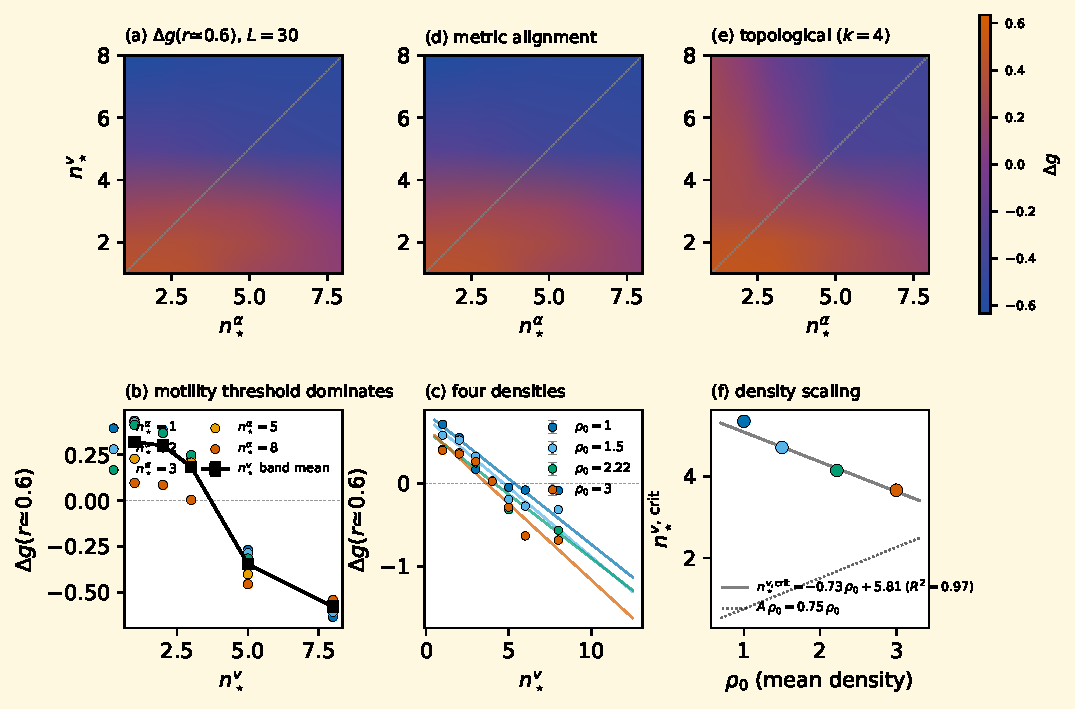
\includegraphics[width=0.98\linewidth]{fig_double_decoupled_2d.pdf}
    \caption{Decoupled-sigmoid dissection of the gap
    $\Delta g(r\!\simeq\!0.6) = g_{\rm full}^{\rm decoupled} -
    g_{\rm motility}$ at $L = 30$, ten seeds per cell. (a) Heatmap
    on the $(n_\star^\alpha, n_\star^v)$ plane (dashed
    $n_\star^v = n_\star^\alpha$). (b) $\Delta g$ vs $n_\star^v$
    keyed by $n_\star^\alpha$, with band means ($\pm 95\%$ CI)
    crossing zero at $n_\star^v \simeq 4$ ($R^2 = 0.88$ on
    $n_\star^v$ vs $0.04$ on $n_\star^\alpha$). (c) Density-scaling
    test at $\rho_0 \in \{1.0, 1.5, 2.22, 3.0\}$ ($n_\star^\alpha =
    3$). (d) Metric and (e) topological ($k = 4$) heatmaps at
    $\rho_0 = 2.22$, matched scale. (f) Critical threshold
    $n^{v,\,{\rm crit}}_\star(\rho_0) = -0.73\,\rho_0 + 5.81$
    ($R^2 = 0.97$; dotted, mean-density prediction $A\rho_0$).}
    \label{fig:decoupled_2d}
\end{figure*}

The map splits the quadrant into two horizontal bands,
separated not by the diagonal but by a critical motility
threshold $n_\star^v \simeq 4$, just above the typical
alignment-zone occupancy $\rho_0\pi(R_a^2 - R_r^2) \simeq
1.7$. Averaging each $n_\star^v$ band over $n_\star^\alpha$, the
mean gap steps monotonically from
$+0.32$ ($95\%$ seed-bootstrap CI $[+0.31, +0.33]$) at
$n_\star^v = 1$ down to $-0.58$ ($[-0.59, -0.57]$) at $8$, the
adjacent bands non-overlapping and the sign flipping at
$n_\star^v \simeq 4$, while the matching $n_\star^\alpha$ bands
stay near zero ($+0.03$ for $n_\star^\alpha \le 3$, down to
$-0.16$ at $n_\star^\alpha = 8$): the noise-shape threshold is
passive. The shared-sigmoid diagonal ($n_\star^v =
n_\star^\alpha$) crosses straight from the positive bands at
$n_\star^v \le 3$ to the negative bands at $n_\star^v \ge 5$,
so the sign is set by $n_\star^v$ alone, not by the timing
offset, as a linear fit confirms ($\Delta g \simeq
-0.144\, n_\star^v + 0.52$, $R^2 = 0.88$, against $R^2 = 0.04$
on $n_\star^\alpha$ and $0.28$ on the timing offset).

The mechanism is simple. At $n_\star^v = 3$, just above typical
occupancy, dense-patch particles fire the motility channel while
the rest saturate at $v_{\max}$. Push $n_\star^v$ to $5$ or $8$
and the motility channel almost never fires: the decoupled model
collapses onto the noise-shape-only ablation, which has
$g(r\!\simeq\!0.6) = -0.17$ at $L = 30$ (Sec.~\ref{sec:gr}), so
its gap with motility-only is large and negative, the lower
band. Drop $n_\star^v$ below $3$ and the motility channel
engages aggressively, dense patches grow, and the noise-shape
rectification adds coherence on top whether it triggers early or
late, the upper band. The slowdown is again the precondition.

\label{sec:decoupled-sigma}
How does the critical motility threshold
$n_\star^{v,{\rm crit}}$ move with the global density $\rho_0$?
The mean-density reading takes the relevant count to be $A\rho_0
= \pi(R_a^2 - R_r^2)\,\rho_0$ and predicts $n_\star^{v,{\rm
crit}} \propto \rho_0$ with slope $A \simeq +0.75$. Sweeping
$n_\star^v \in \{1, 2, 3, 4, 5, 6, 8\}$ at $\rho_0
\in \{1.0, 1.5, 2.22, 3.0\}$, $n_\star^\alpha = 3$ fixed, ten
seeds, we read the zero crossing of $\Delta g(n_\star^v)
\simeq a(\rho_0)\, n_\star^v + b(\rho_0)$. Per-density fits all
reach $R^2 \ge 0.86$ (Fig.~\ref{fig:decoupled_2d}c) and
\begin{equation}
n_\star^{v,{\rm crit}}(\rho_0)
   = -0.73\,\rho_0 + 5.81,
\qquad R^2 = 0.97.
\label{eq:nv_crit_sigma}
\end{equation}
The mean-density prediction is wrong in sign:
$n_\star^{v,{\rm crit}}$ falls with $\rho_0$, the slope
$-0.73$ the mirror image of $+0.75$.

The reversed sign most likely traces to the dense-to-dilute
density contrast, a phenomenological reading we leave for a
first-principles account (App.~\ref{sec:hydro}). At low $\rho_0$
the dilute phase is nearly empty, so the dense phase carries a
large relative contrast and its local count clears even a
demanding $n_\star^v \simeq 5$; at high $\rho_0$ the dilute
phase is itself crowded, the contrast weakens, and $n_\star^v$
must drop to stay selective. Extrapolating
Eq.~\eqref{eq:nv_crit_sigma} to $\rho_0 \simeq 8$ gives
$n_\star^{v,{\rm crit}} \to 0$: once the two phases are
indistinguishable, no threshold buys a coherence gain. The
naive alternative is falsified, since if $n_\star^{v,{\rm crit}}$
tracked the dense-phase neighbour count $\langle n_i\rangle_{\rm
dense}$ the two would be equal, yet $\langle n_i\rangle_{\rm
dense}$ \emph{increases} with $\rho_0$ ($2.6$ at $\rho_0 = 1.0$
to $5.3$ at $\rho_0 = 3.0$), opposite to $n_\star^{v,{\rm
crit}}$.


\label{sec:decoupled-topo}
Metric alignment conflates two roles: the sigmoid input $n_i$
and the partner set are the same object. We pull them apart with
the topological variant of \citet{Ginelli2010}, each
particle aligning with its $k$ nearest non-repulsion neighbours
while the sigmoid input stays the metric annulus count.
Re-running the $25$-cell map at $L = 30$, $\rho_0 = 2.22$ with
$k = 4$ (Fig.~\ref{fig:decoupled_2d}e), the two-band structure
softens: the linear fit on $n_\star^v$ alone drops from $R^2 =
0.88$ to $0.68$ while the $n_\star^\alpha$ fit climbs from
$0.04$ to $0.43$, the bivariate fit now splitting its weight
nearly evenly, and the sign-flip region retreats, cells once
strongly negative under metric alignment turning positive,
only the high-high corner staying negative.

So motility-threshold dominance is a property of the metric
kernel, not of the two-feedback dynamics. Under metric alignment
$n_{\rm ali}$ both feeds the sigmoid and selects the alignment
partners, so pushing the threshold above typical occupancy
switches off the slowdown and the neighbour-driven alignment at
once; topological alignment breaks that tie, the $k = 4$ nearest
neighbours handing each particle a baseline alignment the
rectification can sharpen even when the motility channel is
nearly silent.

\label{sec:decoupled-lifetime}
The full-mode droplets are larger; are they longer-lived? We
track the centroids of the connected dense components over $200$
snapshots spaced $50$ steps, matching across snapshots by
periodic-centroid distance (cutoff $4.0$) and particle-count
ratio (cutoff $2.0$), ten seeds. The mean patch lifetime is
$1.60$ snapshots in motility-only against $1.57$ in the full
mode, a difference of $-0.034$ ($95\%$ bootstrap CI $[-0.10,
+0.03]$, Mann-Whitney $p = 0.08$; not significant); with mean
lifetimes barely above the one-snapshot matching resolution, this
null bounds any persistence difference rather than resolving
sub-snapshot dynamics. The geometric consolidation buys no
temporal persistence: the rectification reshapes which cells the
dense particles occupy at each instant while leaving cell
turnover to the motility dynamics.

Together the four tests pin the rectification down: a spatial
consolidation that needs an aggressive motility threshold and a
metric kernel to engage, works regardless of the noise-shape
threshold, never extends patch lifetimes, and switches off once
the dense-to-dilute contrast washes out, piggybacking on the
MIPS instability rather than driving the phase separation.

\section{Discussion}
\label{sec:disc}

\subsection{Mechanism and biological reading}
\label{sec:disc-mechanism}

What ties the two channels together is the shared sigmoid in
$n_i$: speed and stability index move in lockstep. Inside a
dense patch the sigmoid pushes $\alpha_i \to 2$, replacing the
Cauchy bursts that would otherwise scramble a slow particle by
Gaussian-like kicks. A rectified kick no longer randomises the
local alignment, so the noise-shape channel acts as a
fluctuation rectifier \emph{inside} the slow region the motility
channel carves out. That is the whole of what it does: it lowers
the effective angular noise in the dense phase, and every
advantage of the full mode over motility-only is that single
effect read out in a different observable. The
dense $g(r)$, its dynamic counterpart $C(\tau)$, the
$s_{\rm sep}$ surplus and the finite-size susceptibility excess
all express it, flat in the dilute quartile, and a matched-noise
control removes the full-mode advantage from all of them at once
(Table~\ref{tab:matched}): equalising the dense decorrelation
$\Gamma$ drives $\Delta_9$ from $+0.45$
to $+0.02$ and reverses the $g(r)$ and
$C(\tau)$ gaps as the global retune over-quiets the dilute phase.
The two adaptations therefore do not
cooperate beyond their noise levels; they share one local route,
and at matched noise they simply add. The
decoupled-sigmoid tests of Sec.~\ref{sec:decoupled} sharpen the
picture: the rectification is a spatial consolidation, not a
temporal stabilisation ($p = 0.08$); it needs the metric kernel
($n_\star^v$ dominance weakening from $R^2 = 0.88$ to $0.68$
under topological alignment); the motility threshold controls it
alone; and it switches off once the dense-to-dilute contrast
washes out ($n_\star^{v,{\rm crit}} \to 0$ as $\rho_0 \to 8$).

The biological reading carries an unambiguous priority. A flock
that slows down aggressively reaps the two-feedback cohesion at
almost any noise-shape threshold, whereas one with an inert
motility channel lets the noise-shape adaptation damage
dense-phase coherence. Being a property of the
metric kernel (Sec.~\ref{sec:decoupled}), this priority applies to
short-range metric perceivers such as marching locusts
\citep{Buhl2006, Bazazi2008} and dense bacterial colonies, where
collective motion and cluster formation are set by short-range
contacts \citep{Zhang2010, Peruani2012}, and not to the
topological flockers whose alignment reads a fixed neighbour
number and whose correlations are correspondingly scale-free
\citep{Ballerini2008, Cavagna2010, Ginelli2010}.

\subsection{Literature, limits and outlook}
\label{sec:disc-literature}

The motility channel inherits directly from
\citet{CatesTailleur2015}: our motility-only ablation reproduces
$\partial \ln v / \partial \ln \rho < -1$ MIPS inside an
aligning Couzin flock, with $s_{\rm sep}$ rising from $\simeq
1.2$ for the fixed-speed references to $\simeq 1.7$. This is in
the spirit of \citet{Bi2016}'s density-driven epithelial
jamming, but we keep the alignment interaction, so the dense
phase is polar rather than amorphous. Within the metric-Vicsek
lineage of \citet{Vicsek1995}, \citet{Gregoire2004} and
\citet{Chate2008} established traveling bands and a weakly
first-order transition; the band-soliton index $b \le 1.06$
(Fig.~\ref{fig:profile}) shows we never reach that regime, and
$P(\langle\varphi\rangle)$ stays unimodal at $L = 30$ with $U_4
\simeq 0.65$ in both modes (this single-$\eta$, long-trajectory
cumulant differs from
the $\eta$-resolved minimum of Fig.~\ref{fig:pilot}d that every
mode drives to the same non-diagnostic $0.28$--$0.31$ dip). The
Toner--Tu programme \citep{TonerTu1995, TonerTu1998,
TonerTu2012}, whose predictions have since been assessed
quantitatively against large-scale simulation
\citep{Mahault2019}, gives the same continuous polar order but,
treating the noise as Gaussian with density-independent variance,
does not anticipate the dense-quartile gap of
Fig.~\ref{fig:gr}; the $\Delta a \simeq +0.4$ gap between the
full and motility-only slopes is a quantitative target for a
density-dependent Toner--Tu closure.

The heavy-tail strand is the second axis. \citet{Reynolds2018},
\citet{Harris2012} and \citet{Ariel2015} document L\'evy
reorientations in foragers, T-cells and swarming bacteria, a
strand motivated in part by the search-efficiency argument of
\citet{Viswanathan1999} and formalised through the anomalous-diffusion
framework of \citet{Metzler2000} and \citet{Zaburdaev2015}. Our
noise-shape ablation tempers the heavy-tail-as-driver picture:
the Cauchy and noise-shape modes carry slopes statistically
indistinguishable from zero, so heavy-tailed reorientations on
their own grow no size-dependent $\chi_{\max}(L)$ at our
density, the alignment averaging in the dense phase washing the
bursts out. The motility channel is necessary, heavy tails alone
not sufficient, and what the noise-shape adaptation buys is a
lower effective noise inside the dense
phase, the one route a matched-noise control isolates. Where
\citet{Couzin2002} treats the zonal parameters as global
constants, we make the stability index a local field on the same
kernel; \citet{Bechinger2016} and \citet{Marchetti2013} review
and embed such feedbacks hydrodynamically, but neither
identifies the dense-phase Gaussian conversion, because neither
couples the noise distribution to the local density, and the one
framework general enough to accommodate it leaves that
dependence unexplored by design \citep{Clusella2021}.

Each ingredient is documented on its own: a density-dependent
speed across active colloids, traffic and jamming
\citep{CatesTailleur2015, Greenshields, Bi2016, Angelini2011},
and environment-dependent reorientation statistics in swimming
and swarming bacteria \citep{Korobkova2004, Dieterich2008,
Berg1972}. The closest concrete instance of the two responses
coexisting under one cue is the dense \emph{E.~coli} suspension of
\citet{Colin2019}, where raising cell density both changes the
swimming speed and accelerates heading decorrelation through
collective reorientations; density also tunes the L\'evy exponent
of swarming trajectories \citep{Beer2020} and the reversal
frequency of \emph{M.~xanthus} \citep{Shi1996}. None of this
validates our gate, and it fails to on two counts. The measured
density-dependence of speed in bacterial systems has the opposite
sign to ours, rising rather than falling with crowding
\citep{Colin2019, Beer2020}; and what those experiments resolve is
the reorientation \emph{rate}, not the tail shape of the turning
distribution, the Gaussian-to-heavy-tailed switch in swarms being
controlled by cell aspect ratio rather than by density
\citep{Ilkanaiv2017, Beer2020}. The shared sigmoid is therefore a
deliberate limiting case, not a parsimony claim about any
organism. Its sharpest prediction is a dense-phase narrowing of
the turning-angle distribution together with a positive
heading-correlation gap at fixed effective decorrelation, which an
experiment on a crowding-responsive collective could test, and the
sign of the speed response would have to be established alongside
it.

The weakest part of the case remains the lever. Extending the
scan to $L = 180$ and $256$ lowers both motility-active slopes
($a_{\rm full}: +1.95 \to +1.49$, $a_{\rm motility}: +1.29 \to
+1.04$) and shrinks the each-own-$\eta$ excess ($\Delta_7 = +0.63$
to $\Delta_9 = +0.45$), so the slopes are still drifting on this
window rather than settling, and the matched-noise control then
shows that even the residual excess is a noise-level effect
($\Delta_9 \to +0.02$ on the same nine sizes) rather than a
thermodynamic cooperation. The comparison with the standard
Vicsek value $\gamma/\nu = 1.45(2)$ \citep{Baglietto2008,
Baglietto2012} cuts both ways. The full-mode slope agrees with it
while the motility-only slope does not, which is reassuring as a
consistency check; but with $\eta^\ast(L)$ still migrating, no
collapse available and the window straddling $L^\ast \simeq 128$
\citep{Chate2008}, we make no claim to have measured a critical
exponent. The qualitative split is what survives, and it survives
away from $\rho_0 = 2.22$ as well, so it is not a
parameter-window effect either (Table~\ref{tab:density}). An
explicit data collapse still eludes us, and mapping $g(r)$ at
intermediate distances $r = 2$ to $5$ would tell whether the
rectification carries a characteristic decay length; the absence
of a traveling band leaves room for a different cohesive
structure, perhaps a slowly-rotating dense droplet, that a
real-space analysis at $L > 30$ should reveal. On the theory
side, a
Toner--Tu closure with $v_{\rm eff}(\rho)$ and a fractional
$D_{\rm rot}(\rho) \propto \eta^{\alpha(\rho)}$ recovering both
the linear $\Delta g(n_\star^v)$ and the negative slope
$n_\star^{v,{\rm crit}}(\rho_0) = -0.73\,\rho_0 + 5.81$ would
close the mechanistic argument.

\appendix

\section{A heuristic hydrodynamic sketch and the decoupled-sigmoid asymmetry}
\label{sec:hydro}

The model coarse-grains to fields $\rho(\mathbf x, t)$ and
$\mathbf p(\mathbf x, t) = \rho^{-1}\langle\vec e_i\rangle_x$.
The treatment is heuristic, making the rectification
analytically transparent rather than deriving it.

\subsection{Continuum fields and conservation}
\label{sec:hydro_fields}

With the continuum neighbour count $n_i \approx A\,\rho$,
$A \equiv \pi(R_a^2 - R_r^2) \simeq 0.75$,
Eqs.~\eqref{eq:sigmoid}--\eqref{eq:alpha_adapt} become density
fields,
\begin{align}
\sigma(\rho) & = \frac{1}{1 + \exp\!\bigl[-s\,(A\rho - n_\star)\bigr]},
\label{eq:sigma_rho} \\
v(\rho) & = v_{\max} - \Delta v\,\sigma(\rho),
\quad \Delta v \equiv v_{\max} - v_{\min},
\label{eq:v_rho}
\end{align}
and $\alpha(\rho)$ likewise interpolating from $\alpha_{\min}$
to $\alpha_{\max}$. Density conservation and the polarisation
dynamics read
\begin{equation}
\partial_t \rho + \nabla\!\cdot\!\bigl[\rho\,v(\rho)\,
\mathbf p\bigr] = 0,
\label{eq:rho_eq}
\end{equation}
\begin{equation}
\partial_t \mathbf p = -\Gamma(\rho, \eta)\,\mathbf p
   + \nu\,\nabla^2\mathbf p
   - \lambda\,(\mathbf p\!\cdot\!\nabla)\mathbf p
   + \cdots,
\label{eq:p_eq}
\end{equation}
with $\nu, \lambda$ the standard Toner--Tu coefficients
\citep{TonerTu1995, TonerTu2012}. The non-trivial input is that
the decorrelation rate $\Gamma$ depends on $\rho$ through
$\alpha(\rho)$.

\subsection{Effective rotational decorrelation}

A symmetric $\alpha$-stable kick gives $\langle\cos\xi\rangle =
\exp(-\eta^\alpha)$, so for small $\eta$
\begin{equation}
\Gamma(\rho, \eta) = 1 - \langle\cos\xi\rangle
   \;\simeq\; \eta^{\alpha(\rho)}.
\label{eq:gamma_eta}
\end{equation}
This is $\eta$ in the dilute (Cauchy) limit and $\eta^2$ in the
dense (Gaussian) one, the noise-shape feedback turning the
$\eta$-linear Cauchy decorrelation into the much weaker $\eta^2$
Gaussian one inside the dense phase, the analytic counterpart of
the rectification.

Because the kick enters the heading only modulo $2\pi$, the form
$\langle\cos\xi\rangle = \exp(-\eta^\alpha)$
is exact rather than small-$\eta$: it is the mean resultant length
of the wrapped symmetric $\alpha$-stable law
\citep{Gatto2003, Pewsey2008, Mardia2000}, so it already
integrates the wrapping, and $\Gamma \to 1$ as $\eta^\alpha$ grows, the
wrapped kick saturating to the uniform circle. The heavy
tail acts through the fraction of kicks that overshoot a half-turn
and wrap, $P(|\xi| > \pi) = 1 - (2/\pi)\arctan(\pi/\eta) \simeq
(2/\pi^2)\,\eta \approx 0.20\,\eta$ in the Cauchy limit
($1.0\%, 2.0\%, 4.0\%, 6.1\%$ at $\eta = 0.05, 0.1, 0.2, 0.3$),
against $< 10^{-11}$ for the Gaussian one at the same $\eta$: a few
per cent of every Cauchy step is a near-uniform reorientation the
Gaussian channel never produces. Driving $\alpha$ from $1$ to
$2$ inside the motility-built dense phase removes precisely this
wrapped-uniform fraction, the microscopic content of the
rectification and the reason the dense-phase turning tail
(Fig.~\ref{fig:dynamics}c) collapses onto a Gaussian core while the
dilute gas keeps its L\'evy reorientations.

\subsection{MIPS instability and its rectification correction}

A homogeneous polar state goes unstable under a longitudinal
density perturbation by the Cates--Tailleur mechanism
\citep{CatesTailleur2015} when
\begin{equation}
\frac{\partial \ln v(\rho)}{\partial \ln \rho}\bigg|_{\rho_0}
   < -1,
\label{eq:CT_criterion}
\end{equation}
which the sigmoidal $v(\rho)$ meets in a window of width $1/s$
centred on $A\rho_0 \simeq n_\star$. Since $v$ and $\alpha$
share the sigmoid, that window coincides with the density at
which the rectification fires, so the nucleating dense phase is
born already rectified.

The sketch has a real limit. A sequential timing argument
predicts only the diagonal ordering of the decoupled map,
whereas the data run along horizontal lines of constant
$n_\star^v$ (Fig.~\ref{fig:decoupled_2d}, $R^2 = 0.88$ against
$0.28$ for the timing-offset fit). Neither the horizontal-band
structure nor the negative slope $n_\star^{v,{\rm
crit}}(\rho_0) = -0.73\,\rho_0 + 5.81$ follows from the
linear-stability picture; recovering both would need the
dense-phase density tied to the MIPS contrast rather than the
mean, which we leave to a quantitative theory.

\section*{Code and data availability}
The simulation code, all run drivers, the
figure-generation scripts and the precompiled data are openly
available at
\url{https://github.com/yayayou47/two-feedback-vicsek} under
the \textsc{mit} license. The commit corresponding to this
manuscript carries the tag \texttt{jstat-submission}, so the
exact version underlying every figure can be retrieved
unambiguously. All runs used
Python~3.12.3, NumPy~2.4.4, SciPy~1.17.1, Numba~0.65.1
(LLVM~0.47.0) and Matplotlib~3.10.9 on Linux x86\_64. The
interaction loop is JIT-compiled with Numba's parallel
reduction; per-particle random streams are derived from a
single NumPy \texttt{Generator} with a per-run seed, so
each \texttt{(seed, mode, $L$)} tuple is reproducible
bit-for-bit.

% =====================================================================
%  DÉCLARATION D'USAGE D'IA — EXIGÉE PAR JSTAT.
%
%  Le guide auteur de JSTAT est explicite : « Authors are required to
%  declare and properly reference in detail the use of AI assisted
%  technology in the preparation of the manuscript, either in the
%  methods or acknowledgments section. »  Elle était absente du paquet.
%
%  Je ne peux PAS la rédiger à votre place : c'est un énoncé factuel
%  sur votre processus de travail, et seul vous savez ce qui a été
%  utilisé.  Choisissez la formulation exacte ci-dessous, décommentez-la,
%  et supprimez les autres.  Ne rien déclarer alors que de l'assistance
%  a été utilisée est un manquement à l'éthique de publication d'IOP.
%
%  (a) Aucune assistance :
%  \section*{Use of AI-assisted technology}
%  No generative artificial-intelligence tool was used in the
%  preparation of this manuscript.
%
%  (b) Assistance rédactionnelle seulement (langue, style) :
%  \section*{Use of AI-assisted technology}
%  A large language model (NAME, VERSION, VENDOR) was used to improve
%  the wording and readability of the manuscript. The authors reviewed
%  and edited all output and take full responsibility for the content
%  of the published article. No text was generated without author
%  verification, and the tool was not used to produce, analyse or
%  interpret any data.
%
%  (c) Assistance à l'analyse ou au code, en plus de la rédaction :
%  \section*{Use of AI-assisted technology}
%  A large language model (NAME, VERSION, VENDOR) was used to assist
%  with the wording of the manuscript and with the drafting and review
%  of analysis scripts. All scientific results, figures and numerical
%  values were produced by the code deposited with this article and
%  were verified by the authors, who take full responsibility for the
%  content of the published article.
% =====================================================================

\bibliographystyle{plainnat}
\bibliography{refs}


\end{document}
